ARIMA (AutoRegressive Integrated Moving Average) is a widely used statistical model for forecasting time series data. It is designed to capture patterns such as autocorrelation and trends in the data.

The model is defined by three parameters: $p$, $d$, and $q$.
\begin{itemize}
    \item $p$: the number of autoregressive (AR) terms, which model the relationship between the current value and its past values.
    \item $d$: the degree of differencing used to make the series stationary.
    \item $q$: the number of moving average (MA) terms, which model the relationship between the current value and past forecast errors.
\end{itemize}

A seasonal extension $(P, D, Q, m)$ can also be included, where $m$ represents the number of time steps in one seasonal cycle. This allows the model to capture repeating patterns that occur every $m$ periods. \\

The optimal parameters are selected by minimizing the Akaike Information Criterion (AIC), which balances model fit and complexity. \\

\subsubsection{SARIMAX}
SARIMAX is an extension of the ARIMA model. The \textit{S} represents the seasonal component introduced previously, while the \textit{X} indicates the inclusion of exogenous input features. Unlike ARIMA, which only models the historical behavior of the time series itself, SARIMAX can additionally incorporate external variables that may influence the forecasting.

\subsubsection{Model Optimization}

The following method was used to validate the ARIMA forecasting approach on the dataset. As described earlier, the data consists of two groups seasonal and non-seasonal. For each individual cell time series, the auto ARIMA function [Put python documentaration link here]  was applied to determine the parameter set that minimizes the AIC. The most frequently selected order across all cells was then chosen as the representative seasonal and non-seasonal configuration. \\

The proposed evaluation procedure consisted of three stages:

\begin{enumerate}
    \item First, the baseline ARIMA configuration was determined using auto-ARIMA without any exogenous variables.
    
    \item Second, forward feature selection was applied to the exogenous variables using the fixed baseline ARIMA order.
        
    \item Finally, after selecting the optimal feature subset, the ARIMA coefficients and
    model parameters were re-estimated using the selected exogenous variables to obtain
    the final SARIMAX model
\end{enumerate}


\subsubsection{baseline ARIMA configuration}

\begin{figure}[htbp]
    \centering

    \begin{subfigure}[b]{0.9\linewidth}
        \centering
        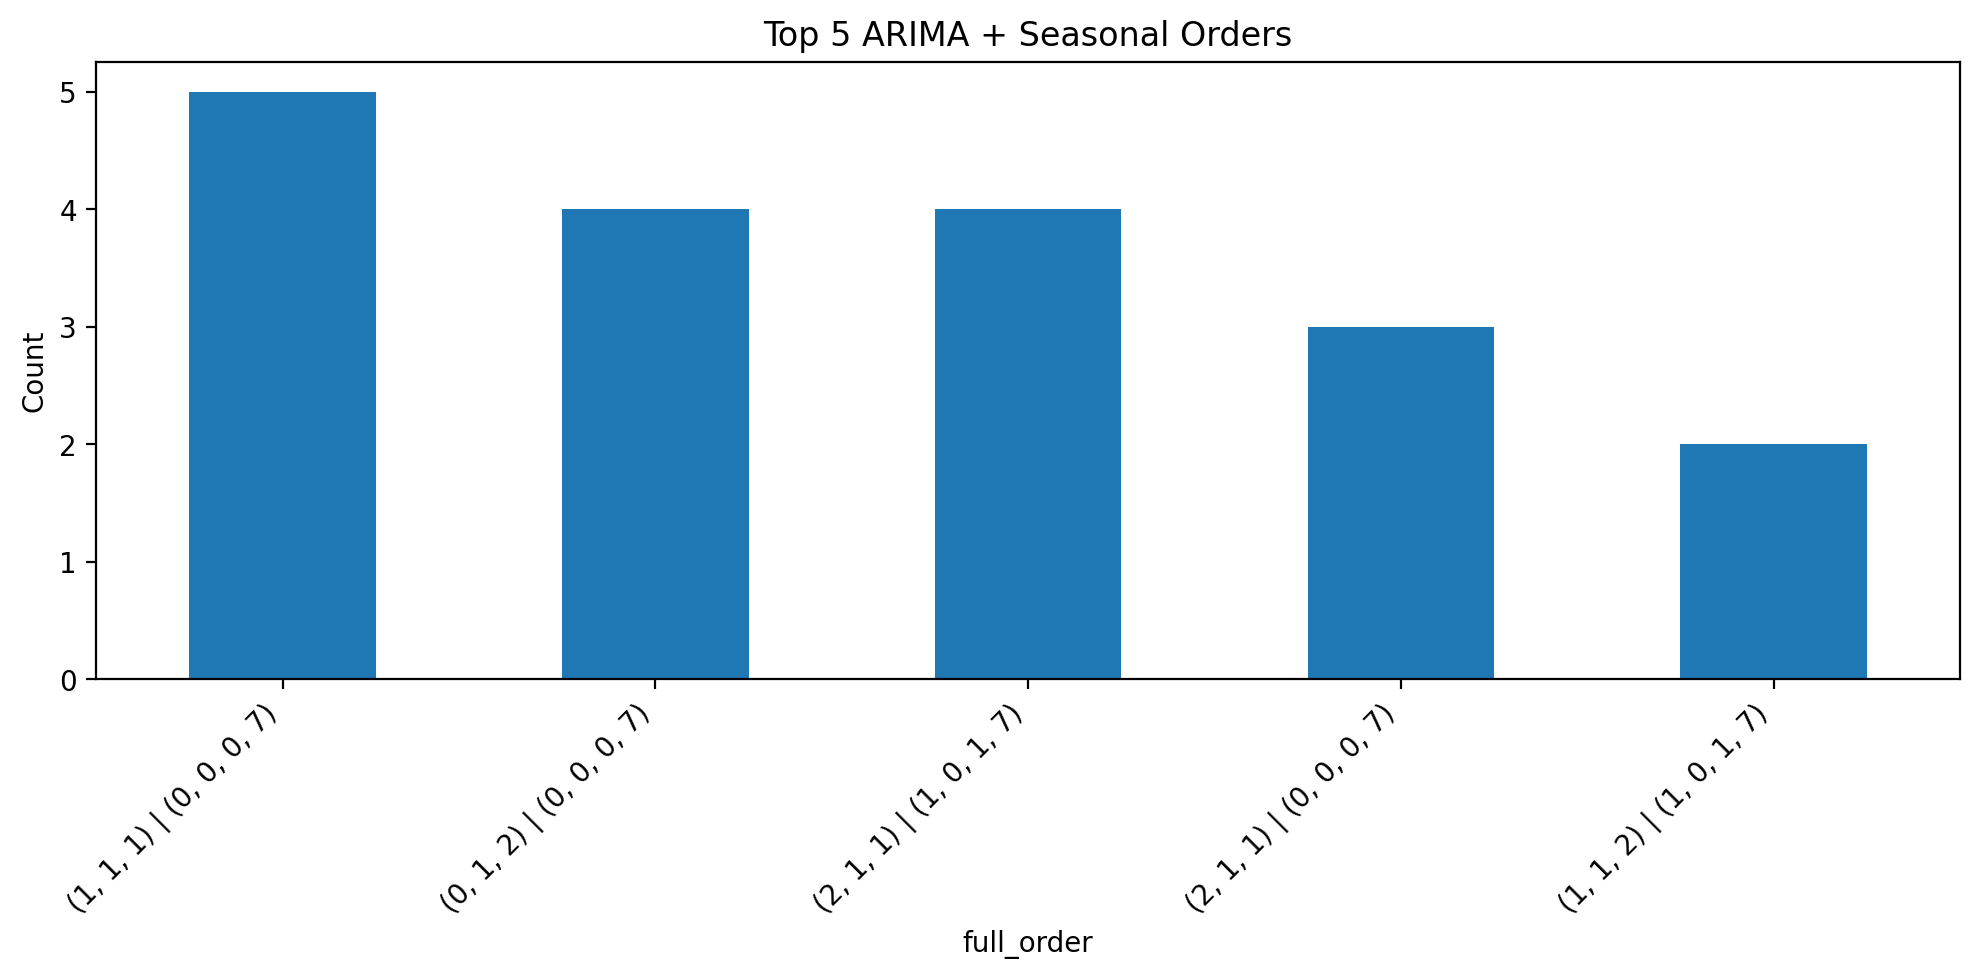
\includegraphics[width=0.9\linewidth]{figures/arima_seasonal_pre_order.png}
        \caption{ARIMA order frequency for seasonal cell}s
        \label{fig:arima_seasonal_pre_order}
    \end{subfigure}

    \vspace{0.5cm}

    \begin{subfigure}[b]{0.9\linewidth}
        \centering
        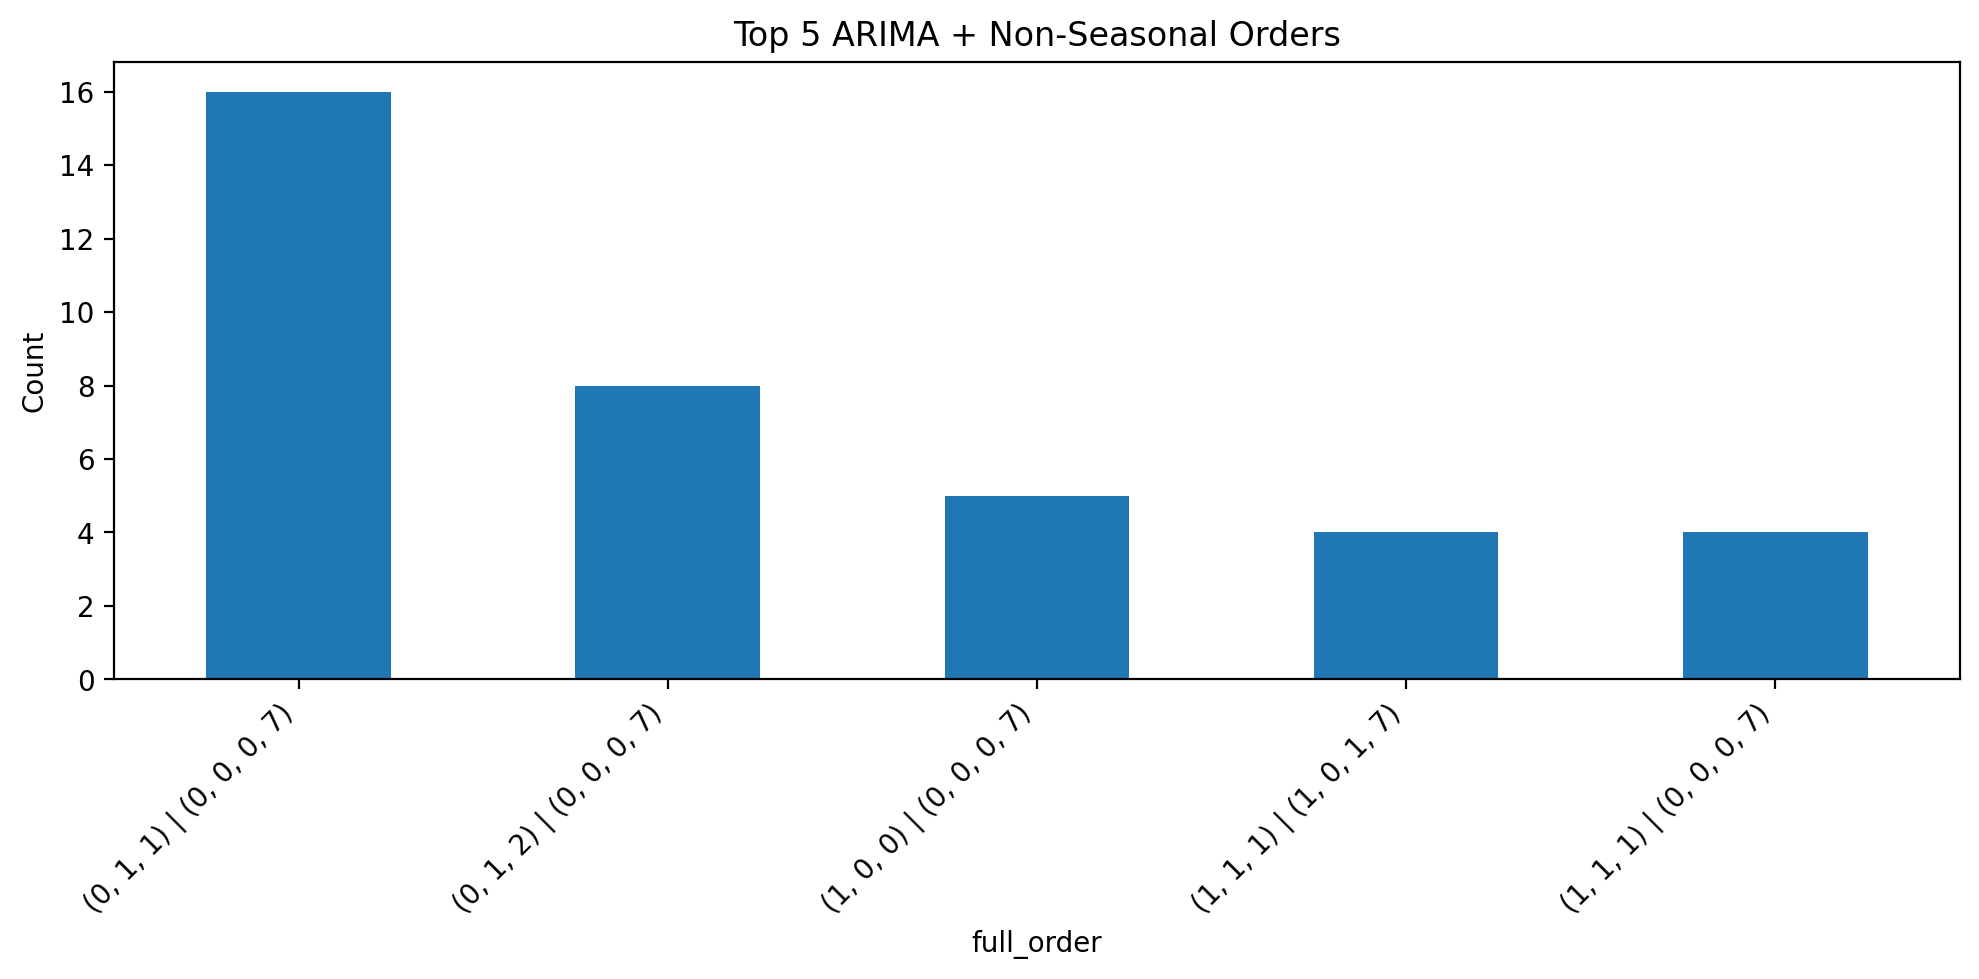
\includegraphics[width=0.9\linewidth]{figures/arima_non_seasonal_pre_order.png}
        \caption{ARIMA order frequency for non-seasonal cell}
        \label{fig:arima_non_seasonal_pre_order}
    \end{subfigure}
    
    \begin{subfigure}[b]{0.9\linewidth}
        \centering
        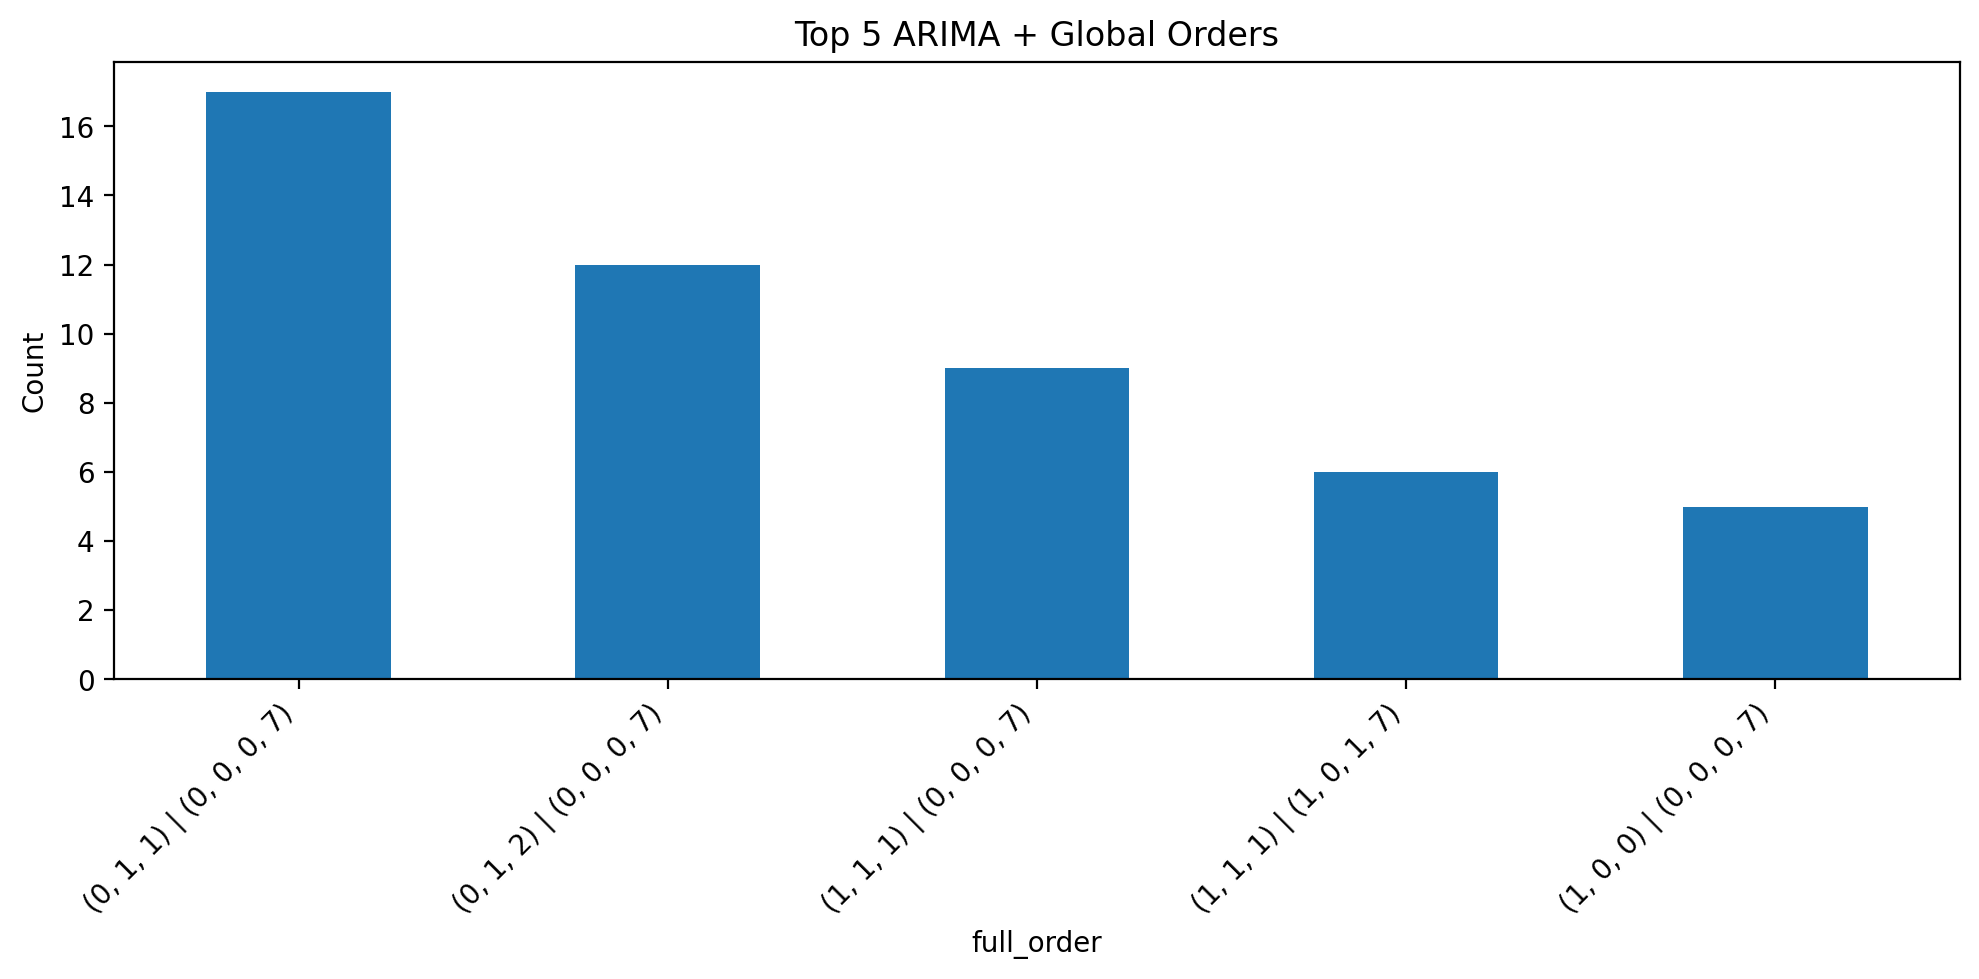
\includegraphics[width=0.9\linewidth]{figures/arima_global_pre_order.png}
        \caption{ARIMA order frequency for all cells}
        \label{fig:arima_global_pre_order}
    \end{subfigure}
    
    \caption{Arima order before feature selection}
    \label{fig:pre_order_arima}
\end{figure}

Figure~\ref{fig:pre_order_arima} shows the frequency of the ARIMA orders selected by the auto-ARIMA procedure across all seasonal cell time series. \\

For the seasonal setting, the most frequently selected configuration was ARIMA$(1,1,1)(0,0,0,7)$. This indicates that first-order differencing was consistently required, while the dominant structure was captured through short-term autoregressive and moving-average components. \\

For the non-seasonal setting, the dominant configuration was ARIMA$(0,1,1)(0,0,0, 7)$. Compared to the seasonal case, the autoregressive component disappeared, suggesting weaker temporal dependence in the non-seasonal cells. However, first-order differencing, the moving-average and seasonal components remained consistently selected across both groups. \\

\subsubsection{Feature selection}
To evaluate the impact of exogenous variables on forecasting performance, a forward feature selection approach was used. The goal was to iteratively build a feature set that minimizes the mean squared error (MSE) across all time series (cells). \\

Table~\ref{tab:tested_features} shows the set of candidate features evaluated during the selection process.

\begin{table}[htbp]
\centering
\caption{Candidate features evaluated during feature selection}
\label{tab:tested_features}

\begin{tabular}{ll}
\toprule
\textbf{Feature} & \textbf{Description} \\
\midrule
month & Month of the year \\
dayofweek & Day of the week \\
is\_weekend & Weekend indicator variable \\
holiday & Public holiday indicator \\
lag1 & Previous day traffic value \\
lag7 & Traffic value from 7 days earlier \\
roll\_mean\_7 & Rolling 7-day mean \\
roll\_mean\_14 & Rolling 14-day mean \\
roll\_std\_7 & Rolling 7-day standard deviation \\
roll\_std\_14 & Rolling 14-day standard deviation \\
roll\_min\_7 & Rolling 7-day minimum \\
roll\_max\_7 & Rolling 7-day maximum \\
lag\_diff\_1\_7 & Difference between lag-1 and lag-7 \\
\bottomrule
\end{tabular}
\end{table}

To evaluate the impact of exogenous variables on forecasting performance, a forward feature selection approach is applied. The method starts with an empty feature set and iteratively adds the feature that yields the largest reduction in average test mean squared error (MSE) across all time series. Candidate features include calendar variables, lag-based features, rolling statistics, and differenced features. The process continues until no further improvement is observed, as shown in Algorithm \ref{alg:algo_1}.\\

\begin{algorithm}[H]\caption{Forward Feature Selection for ARIMA with Exogenous features}
\begin{algorithmic}[1]

\STATE Initialize selected feature set $S \leftarrow \emptyset$
\STATE Initialize remaining features $R \leftarrow \{f_1, f_2, ..., f_n\}$
\STATE Set best error $E_{best} \leftarrow \infty$

\WHILE{$R \neq \emptyset$}
    \STATE $f^* \leftarrow \emptyset$
    \STATE $E^* \leftarrow E_{best}$

    \FOR{each feature $f \in R$}
        \STATE Train ARIMA models with feature set $S \cup \{f\}$ across all series
        \STATE Evaluate mean test error $E_f$
        
        \IF{$E_f < E^*$}
            \STATE $E^* \leftarrow E_f$
            \STATE $f^* \leftarrow f$
        \ENDIF
    \ENDFOR

    \IF{$f^* \neq \emptyset$}
        \STATE Add $f^*$ to $S$
        \STATE Remove $f^*$ from $R$
        \STATE Update $E_{best} \leftarrow E^*$
    \ELSE
        \STATE Stop
    \ENDIF

\ENDWHILE

\end{algorithmic}
\label{alg:algo_1}
\end{algorithm}

The forward selection procedure is applied separately to three model configurations: seasonal cells, non-seasonal cells, and the full dataset. Each configuration follows the same evaluation protocol, where features are added sequentially based on their impact on validation RMSE. The final selected feature set for each configuration is determined when no additional feature yields further improvement. \\
\begin{table}[htbp]
\centering
\caption{Feature selection results across seasonal, non-seasonal, and all-cell models}
\label{tab:feature_selection_all}

\begin{tabular}{lcc}
\toprule
\textbf{Model Type} & \textbf{Selected Features (final step)} & \textbf{RMSE} \\
\midrule
Seasonal cells & roll\_mean\_7, roll\_max\_7 & 1.62 \\
Non-seasonal cells & roll\_min\_7, lag\_1, is\_weekend & 1.71 \\
All cells & roll\_min\_7, lag\_1, lag\_diff\_1\_7 & 1.66 \\
\bottomrule
\end{tabular}
\end{table}

Feature selection results show strong overlap between the non-seasonal and all-cell configurations, which converge to the same optimal feature set. In contrast, seasonal cells rely more on short-term aggregated statistics such as rolling means and maxima, while non-seasonal cells benefit from lag-based and difference features that capture local temporal changes. \\

Across all configurations, performance improvements are primarily driven by short-term dependency features (lag-1 and lag-difference), suggesting that recent history dominates predictive power. Seasonal structure contributes less to overall error reduction, indicating weak or inconsistent periodicity across most cells. \\


\subsubsection{Post feature selection order refinement}

After feature selection, the top ARIMA orders identified during the baseline stage were re-evaluated using the selected exogenous variables. Each configuration was refitted and tested on the held-out dataset, and performance was compared to the feature-selection baseline.

\begin{figure}[H]
	\centering
	
	\begin{subfigure}[b]{0.9\linewidth}
		\centering
		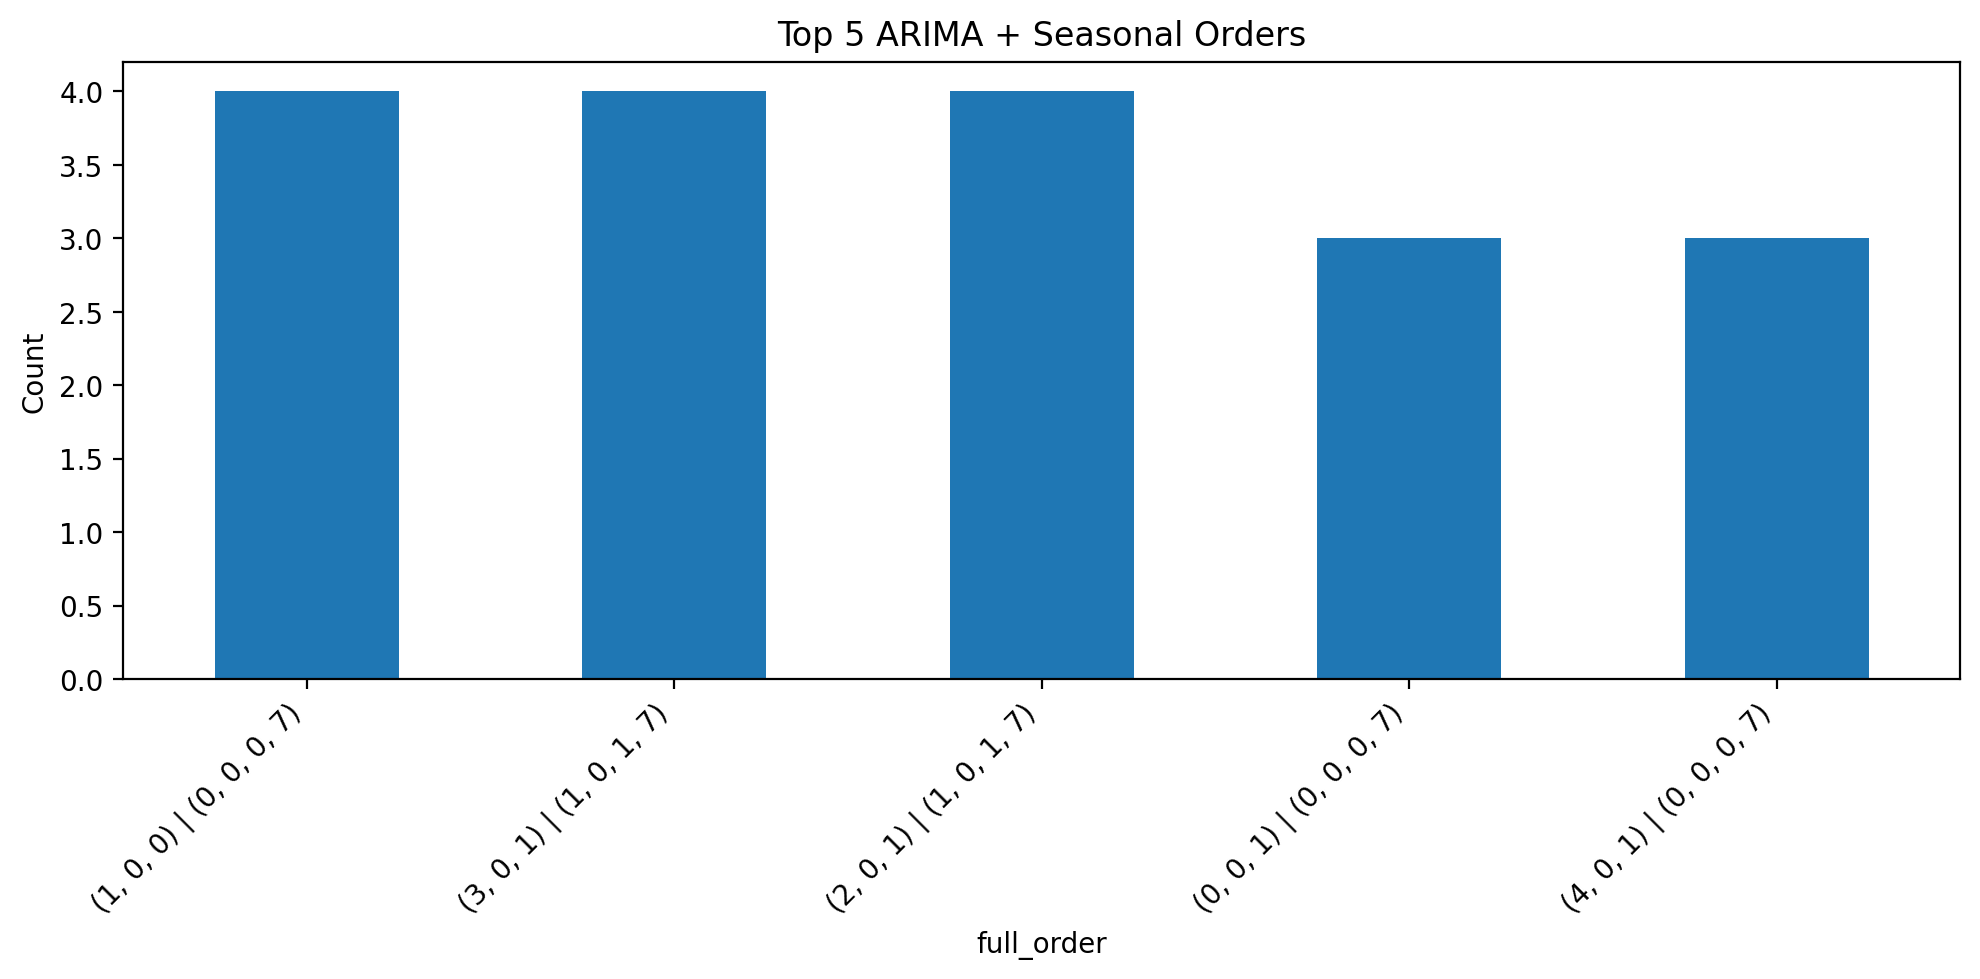
\includegraphics[width=0.9\linewidth]{figures/arima_post_seasonal_order_2.png}
		\caption{ARIMA order frequency for seasonal cells}
		\label{fig:arima_seasonal_post_order}
	\end{subfigure}
	
	\vspace{0.5cm}
	
	\begin{subfigure}[b]{0.9\linewidth}
		\centering
		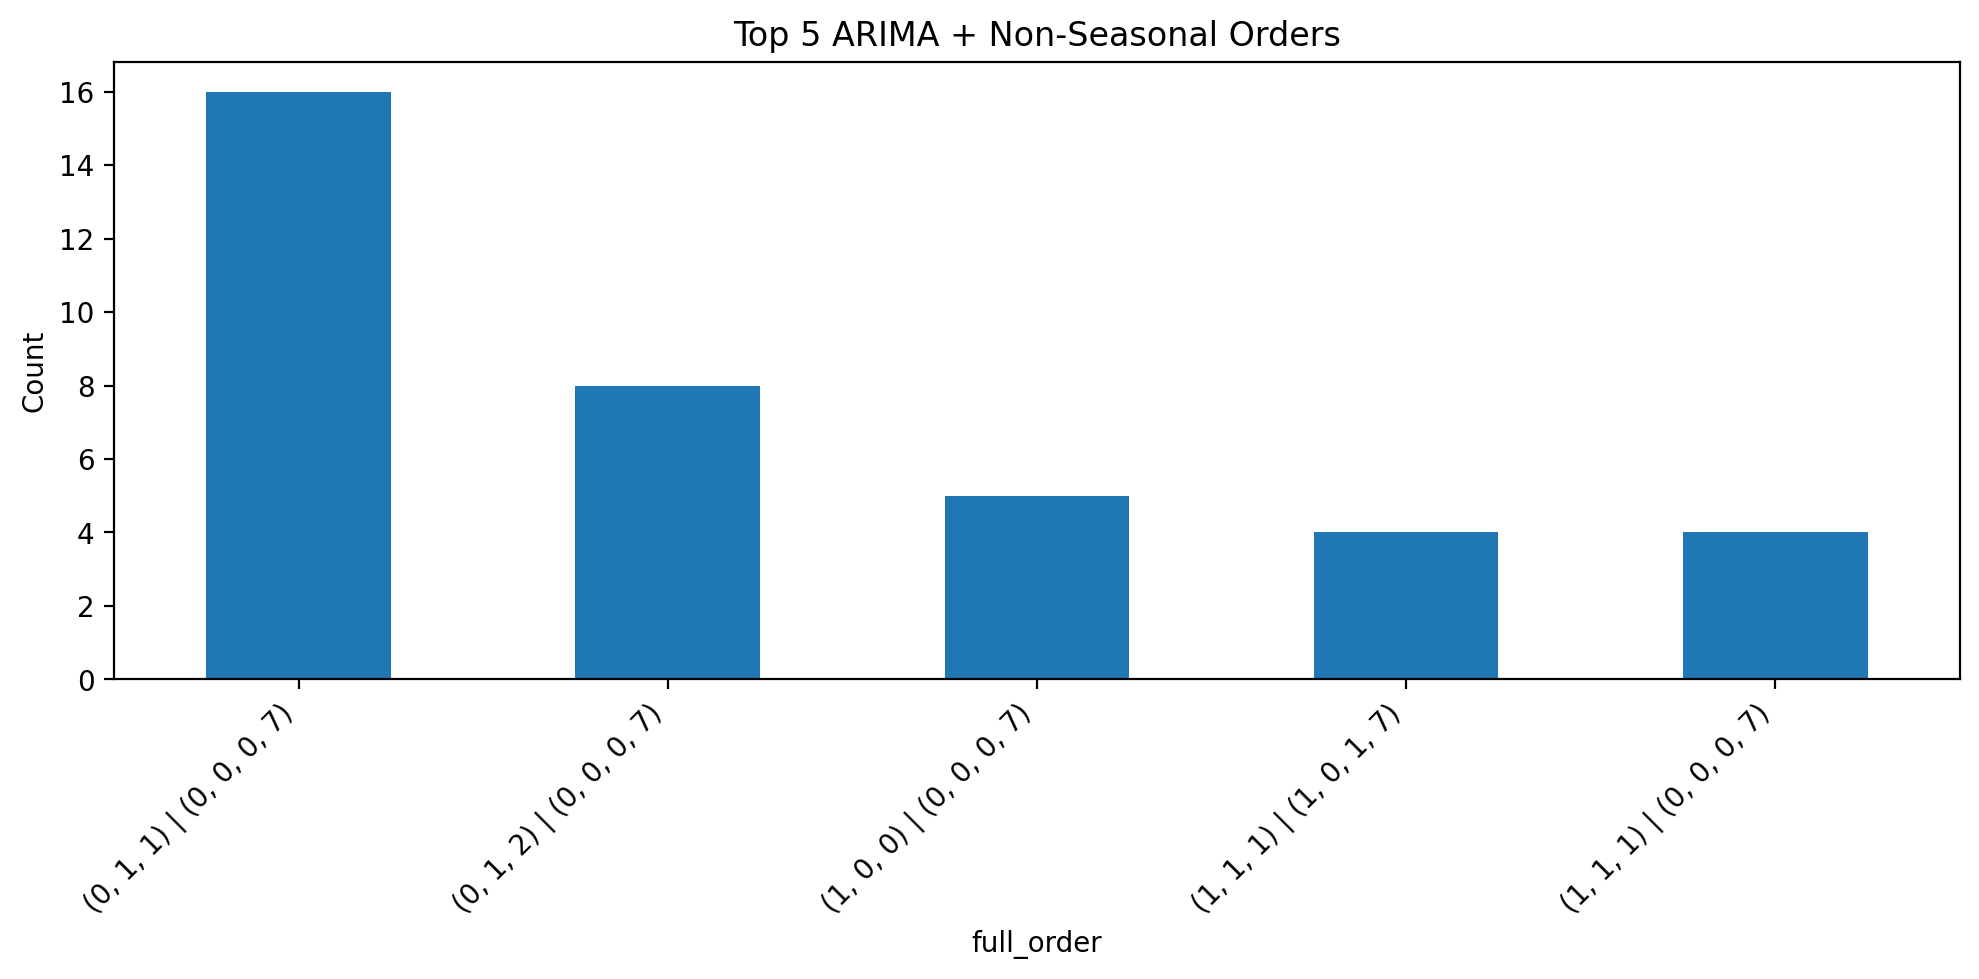
\includegraphics[width=0.9\linewidth]{figures/arima_non_seasonal_pre_order_2.png}
		\caption{ARIMA order frequency for non-seasonal cells}
		\label{fig:arima_non_seasonal_post_order}
	\end{subfigure}
	
	\begin{subfigure}[b]{0.9\linewidth}
		\centering
		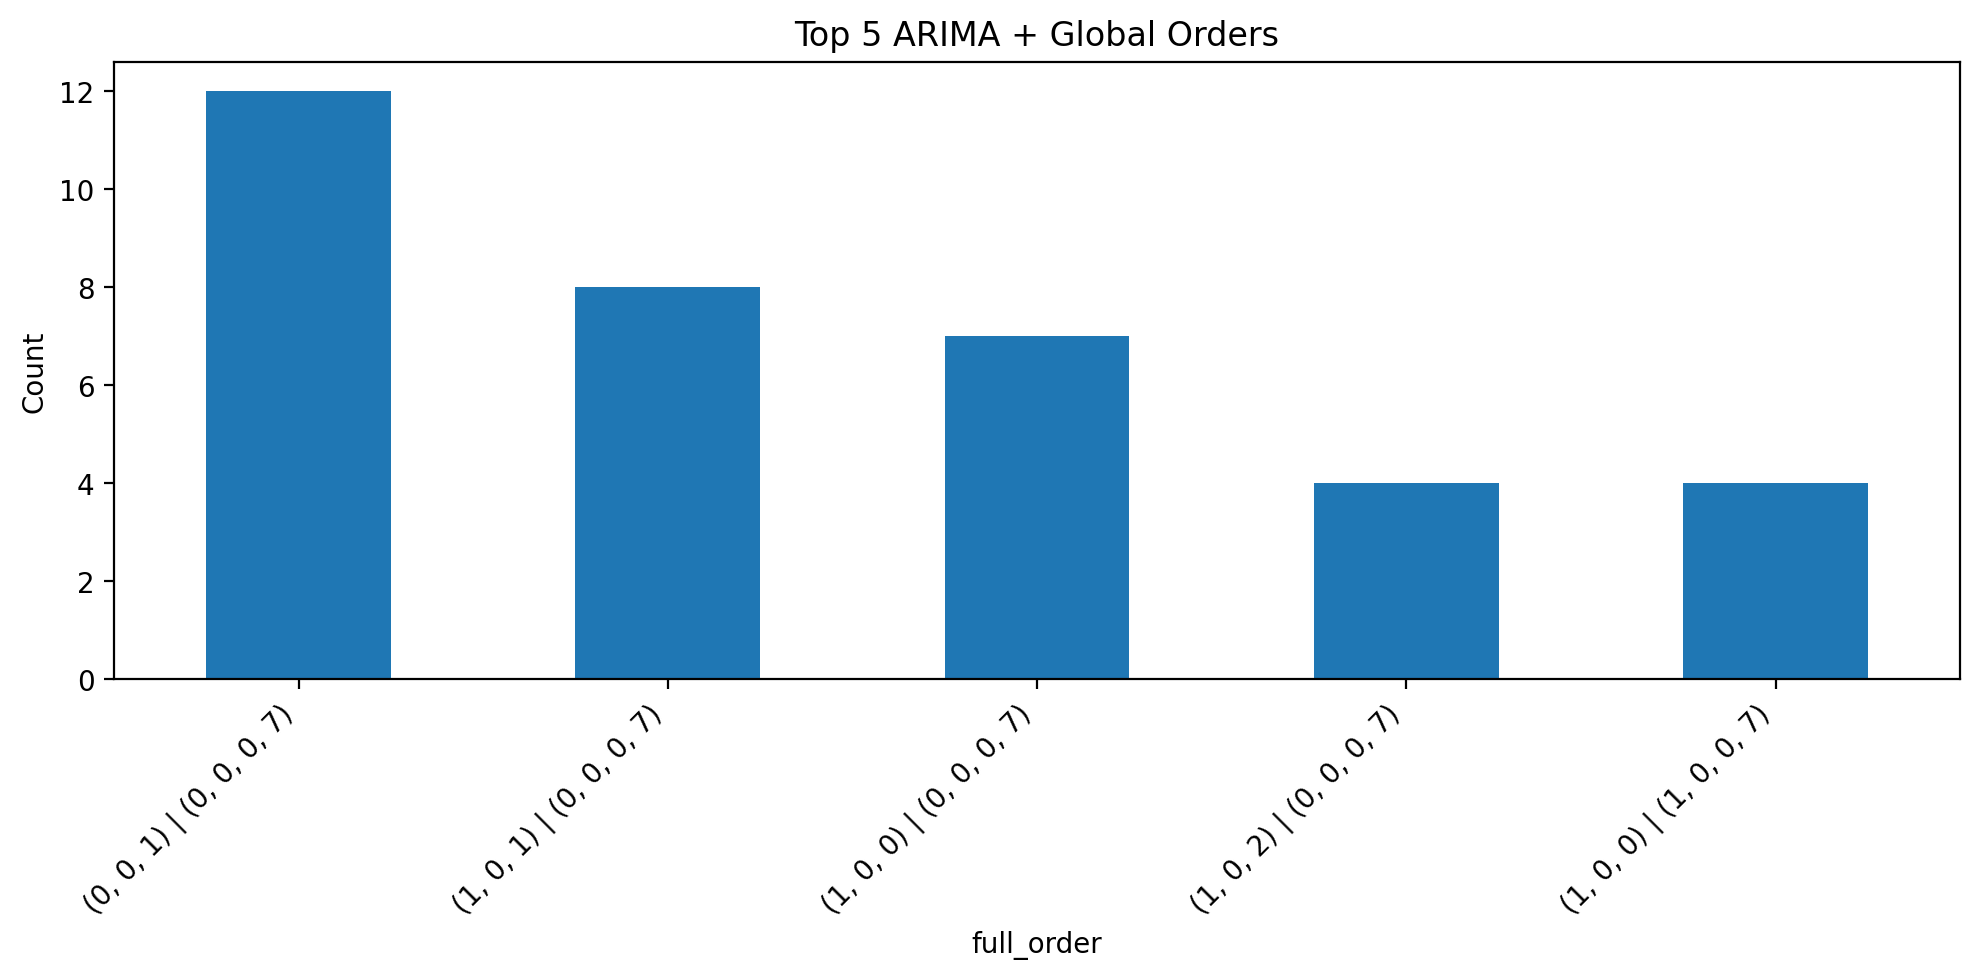
\includegraphics[width=0.9\linewidth]{figures/arima_global_post_order.png}
		\caption{ARIMA order frequency for all cells}
		\label{fig:arima_global_post_order}
	\end{subfigure}
	
	\caption{ARIMA order selection after feature engineering}
	\label{fig:arima_post_orders}
\end{figure}

The results show only limited changes after feature selection. For seasonal cells, a slightly different configuration ARIMA$(0,0,1)(0,0,0,7)$ achieved the best performance with an RMSE of 1.51. For non-seasonal cells and all cells, the original configuration ARIMA$(0,1,1)(0,0,0,7)$ remained optimal.

\begin{table}[htbp]
	\centering
	\caption{Post feature selection ARIMA performance comparison}
	\label{tab:arima_post_results}
	
	\begin{tabular}{lcc}
		\toprule
		\textbf{Model Type} & \textbf{Best Order} & \textbf{RMSE} \\
		\midrule
		Seasonal cells & $(0,0,1)(0,0,0,7)$ & 1.5139 \\
		Non-seasonal cells & $(0,1,1)(0,0,0,7)$ & 1.7102 \\
		All cells (global) & $(0,1,1)(0,0,0,7)$t & 1.6600 \\
		\bottomrule
	\end{tabular}
\end{table}

Overall, the results suggest that both feature engineering and model order selection contribute to forecasting performance. Feature selection provides the main improvement, while re-tuning the ARIMA order after feature selection yields only marginal additional gains. \\

For seasonal cells, a small but consistent improvement is observed after adjusting the ARIMA order, reducing the RMSE from the feature-selection baseline. For non-seasonal and global models, changes in ARIMA order do not lead to meaningful improvements. \\

This indicates that exogenous features carry most of the predictive signal, while ARIMA order tuning provides secondary refinement in certain cases rather than large performance shifts. \\

\begin{figure}[H]
	\centering
	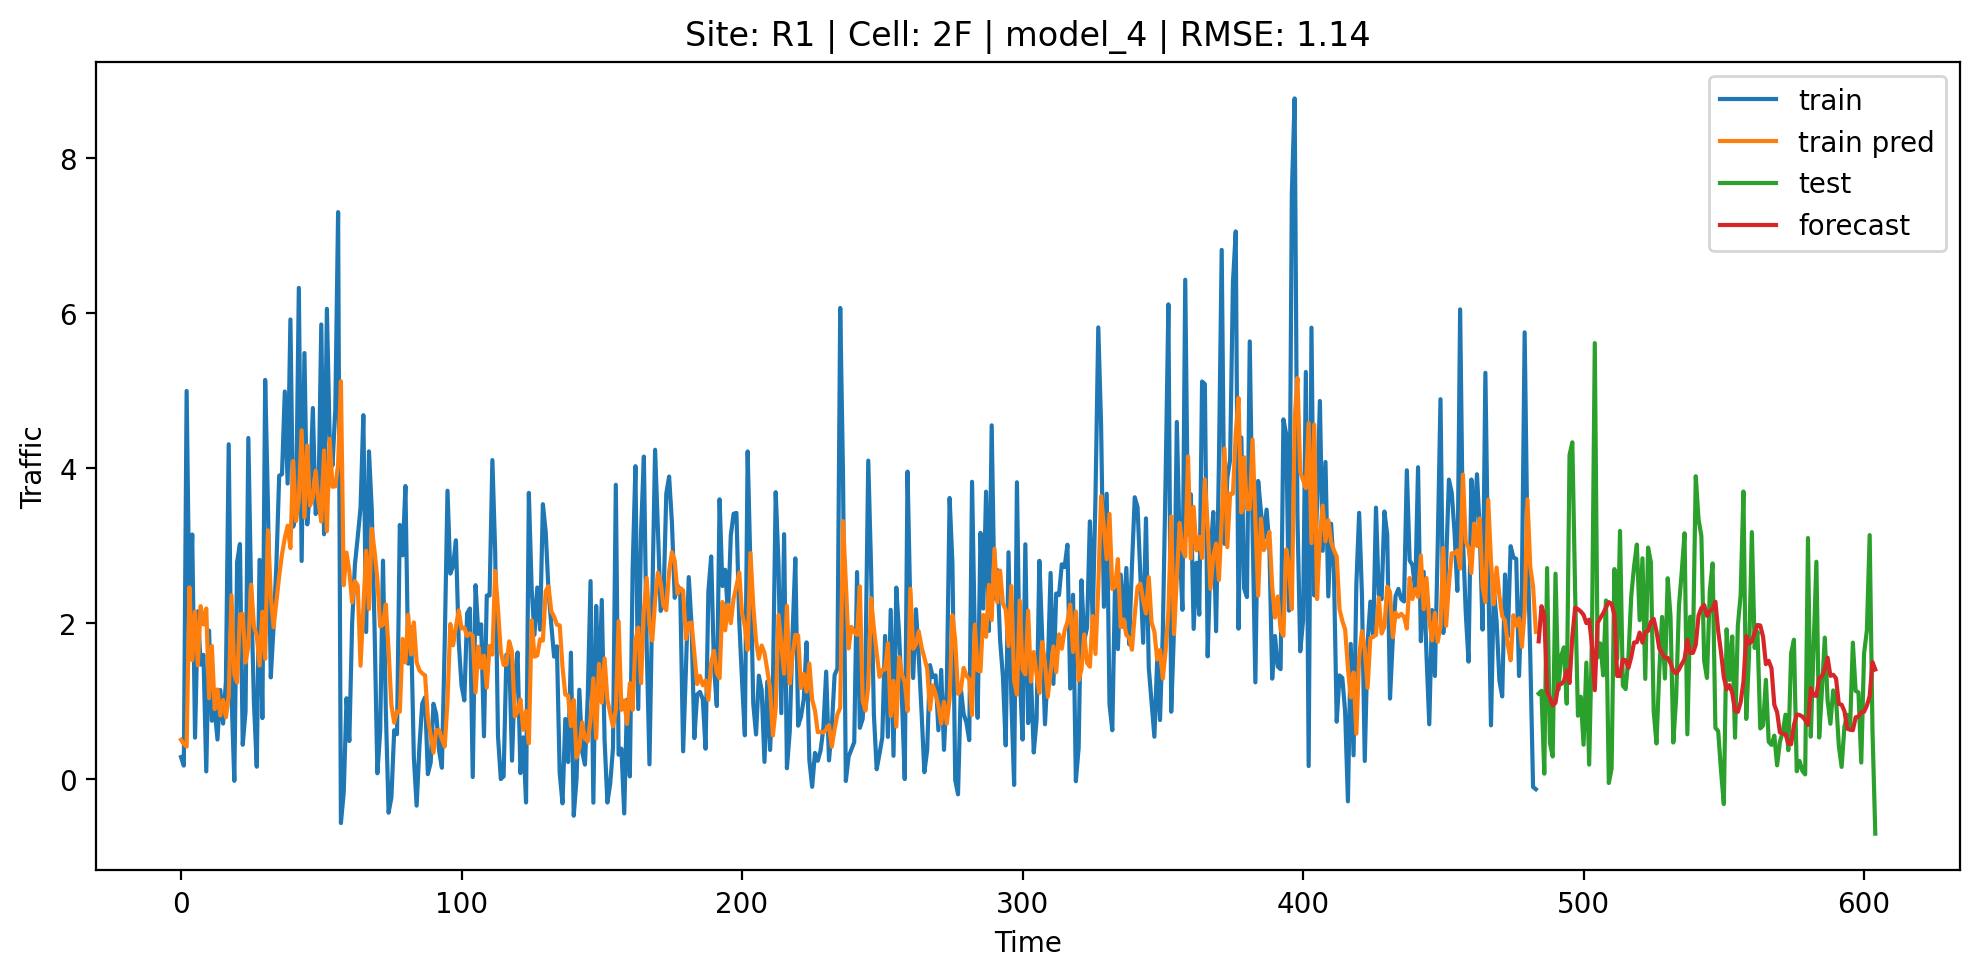
\includegraphics[width=\linewidth]{figures/arima_pred.png}
	\caption{Seasonal Arima Fitting and Prediction on R1 2F}
	\label{fig:arima_prediction}
\end{figure}

To better understand model behaviour, Figure~\ref{fig:arima_prediction} shows the fitted values on the training data and the predictions on the held-out test set for a representative cell (R1, 2F). \\




